\documentclass[a4]{article}
\usepackage{geometry}
\geometry{verbose,tmargin=2.5cm,bmargin=2.5cm,lmargin=3cm,rmargin=3cm}
\usepackage{amsmath,amssymb,amsthm}
\usepackage{graphicx}
\graphicspath{{graphics/}}
\usepackage[utf8]{inputenc}
\usepackage{fancyvrb}
\usepackage{hyperref}
\usepackage{lscape}
\usepackage{adjustbox}
\usepackage{verbatim}
\usepackage{subcaption}
\usepackage{placeins}

\title{MultiFEBE \\ Tutorial 9: harmonic analysis of an offshore wind turbine}
\author{\'A.G. Vega-Artiles}
\date{May 2023}

\begin{document}

\maketitle

\tableofcontents

\part{FEM model of an offshore wind turbine}

\section{Problem description}

In this ninth tutorial, an offshore wind turbine will be studied. In this first part of the tutorial, a FEM model with no soil-structure interaction is considered and unitary horizontal displacements are directly applied at the bottom leg nodes. However, the second part of the tutorial will introduce dynamic soil-structure interaction with the presence of soil and foundations. Figure \ref{fig:geometry1} shows the geometry. Note that the geometry is defined with the z-axis oriented downwards.

\begin{figure}[tbh!]
	\centering
	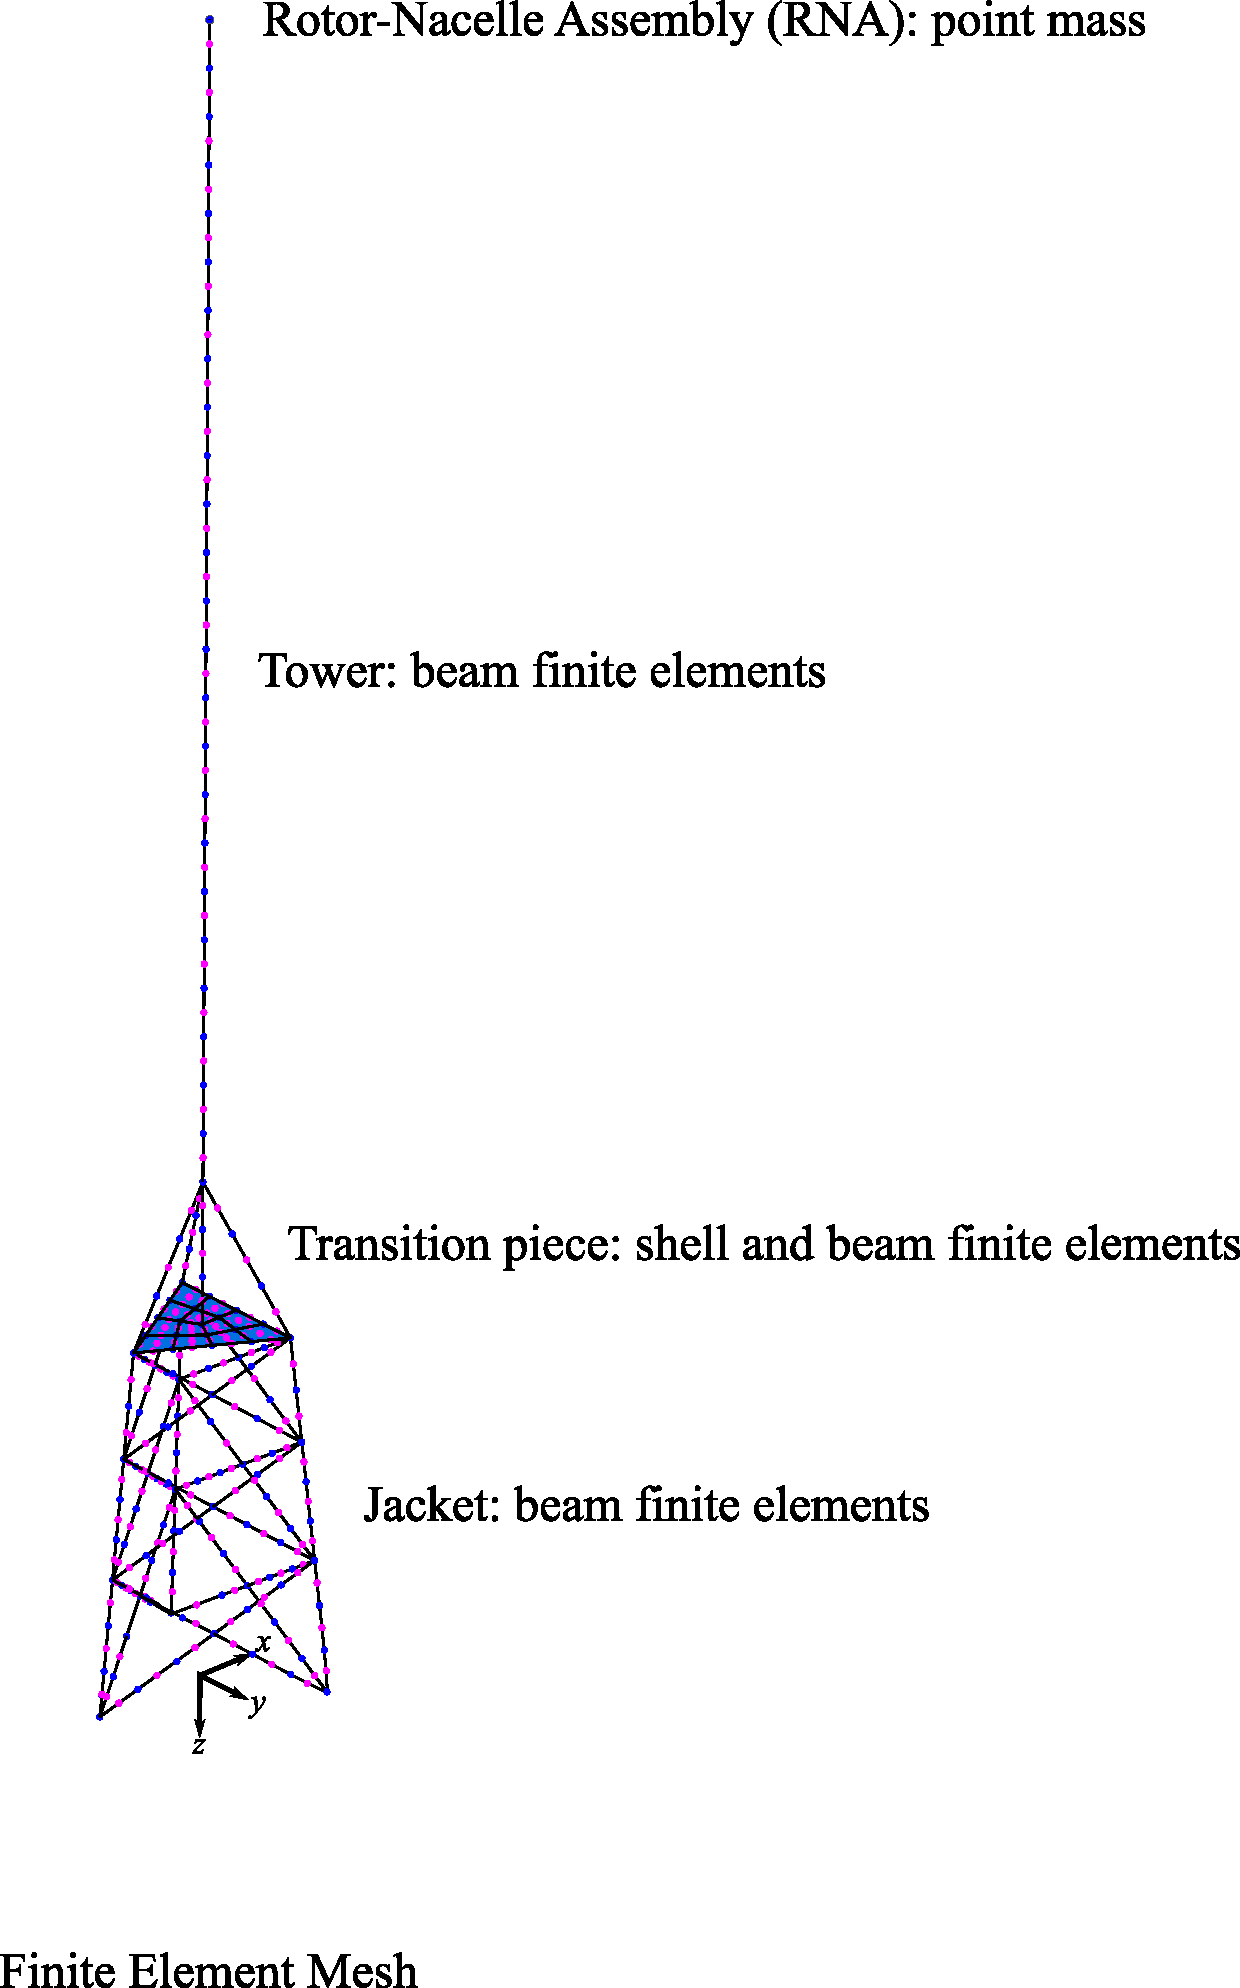
\includegraphics[scale=0.5]{owt_model_rigid.pdf}
	\caption{Geometry for the FEM model.}
	\label{fig:geometry1}
\end{figure}

\section{Pre-processing} 
Pre-processing in MultiFEBE consists of defining the geometry and mesh of the problem. There are three ways to do such definition: directly from the input file (mode = 0), from another file in the native format (mode = 1) or from another file in the Gmsh MSH file format version 2.2 (mode = 2). However, it is preferable to use a *.msh file for relatively large geometries, therefore, this is the syntax explained in the following subsections.
   
\subsection{Mesh generation with Gmsh}
Gmsh \cite{gmsh, gmshweb} is a finite element mesh generator with its own language. The software allows to create the geometry in a “bottom-up” manner, going from the most basic elements (points) to the highest order elements (volumes) or in a “Constructive Solid Geometry” manner (boolean operations) or with a combination of methodologies. Gmsh also allows to define  the so-called “physical groups” which are unmodifiable entities that gather elementary entities as sole entities, where every entity must have a unique tag. On the other hand, the file containing all this geometric definition is the *.geo file whereas the mesh definition is in the *.msh file. 

\subsubsection{GEO file}
The Gmsh language allows to define parameters to use later in the script and comments as every other programming language. 

In this example, several parts of the offshore wind turbine were defined in the *.geo file: Jacket joints, Jacket members, Transition piece and Tower.  

The functions used in the present model have been already explained in previous tutorials. The only new function is "Mesh.Algorithm = 6" that sets the "Frontal-Delaunay 2D meshing algorithm".

\begin{figure}[tbh!]
	\centering
	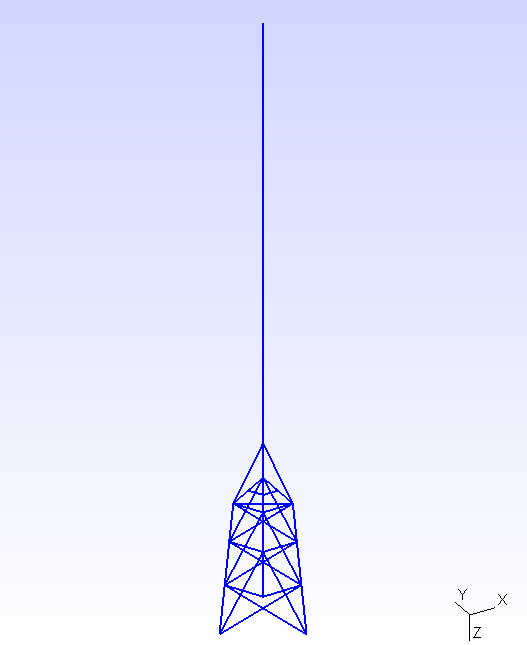
\includegraphics[scale=0.6]{geo1.png}
	\caption{Geometry for the FEM model resulting from the *.geo file.}
	\label{fig:geo1}
\end{figure}

\subsubsection{MSH file}

The *.msh file begins with a mandatory section about information of the file (MeshFormat) and following by the other sections. Here, three sections are used: the physical group names (PhysicalName), the nodes (Nodes) and the elements (Elements).

In the section "PhysicalName", all the physical entities of the model are defined. The first line indicates the number of physical entities. Then, one line per physical entity indicating the physical dimension, the tag and the name.  

In the section "Nodes", all the nodes of the model are defined. The first line indicates the number of nodes. Then, one line per node indicating the identifier of the node and its coordinates (x y z).

In the section "Elements", all the elements of the model are defined. The first line indicates the number of elements. Then, one line per element indicating:

\begin{itemize}
	\item Element identifier.
	\item Type of element.
	\item Number of auxiliary tags.
	\item List of tags, where the two first auxiliary tags are mandatory, and corresponds to the identifier of the physical entity to which the element belongs and the second one is the identifier of the elementary model entity to which the element belongs. The rest of the tags are optional.
	\item A list of identifiers corresponding to the nodes of the element.
\end{itemize}

For example, in this case, an element with the identifiers 2 8 2 2 1 1 51 53 corresponds to:

\begin{itemize}
	\item 2: element 2.
	\item 8: type 8 (3-node second order line).
	\item 2: it has 2 auxiliary tags.
	\item 2: it belongs to the physical entity 1.
	\item 1: it belongs to the line 1.
	\item 1, 51, 53: it connects the nodes 1, 51 and 53.
\end{itemize} 

\begin{figure}[tbh!]
	\centering
	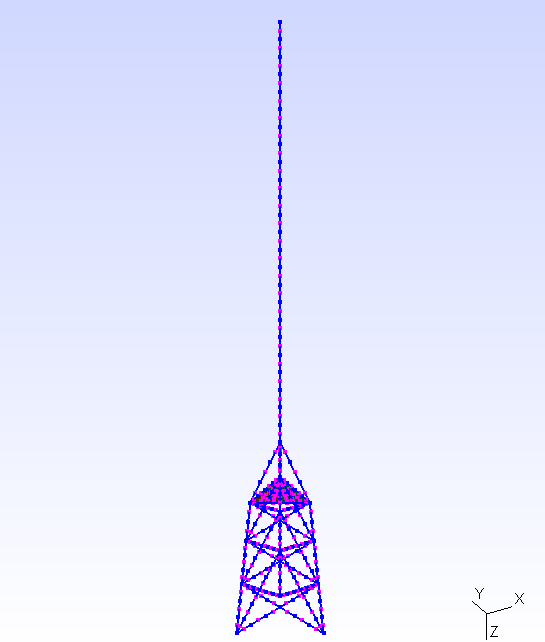
\includegraphics[scale=0.6]{mesh1.png}
	\caption{Mesh for the FEM model resulting from the *.geo file.}
	\label{fig:mesh1}
\end{figure}

\subsection{Input data file}
Solving in MultiFEBE consists of running the software by specifying several options in the following sections\footnote{See reference manual.}: [problem], [settings], [materials], [regions], [conditions over nodes], etc.

The first part to configurate is the problem definition in the section [problem]. This example is a 3D harmonic mechanical problem.

\begin{Verbatim}	
[problem]
type = mechanics
analysis = harmonic
n = 3D
\end{Verbatim}

Then, a list of frequencies is generated by specifying the number of frequencies, that must be $\geq 2$ (200) followed by the minimum frequency $>0$ (0.01) and the maximum frequency (10), being each one in new lines.

\begin{Verbatim}
[frequencies]
Hz
lin
200
0.01
10
\end{Verbatim}

Next step is to configurate the mesh. In this case, a mesh from Gmsh will be used so that it is necessary to write the option number 2 and the document name obtained from it in the section [settings]. However, if the mesh were going to be read from the input file, it would require to write the sections [nodes], [elements] and [parts] instead.

\begin{Verbatim}	
[settings]
mesh_file_mode = 2 "mesh.msh"
\end{Verbatim}

In the section [export], the complex notation is set as cartesian and the format for floating point numbers as Simple Engineering (eng\_simple = en18.8e2) with 18 as the minimum number of positions to be used, 8 the number of digits to the right of the decimal point and 2 the number of digits in the exponent part. 

\begin{Verbatim}
[export]
complex_notation = cartesian
real_format=eng_simple
\end{Verbatim}

As the problem has two materials, the section [materials] will need three lines: a first line for the number of materials in the model and a line per material with its properties such as tag, type, $\rho$, E, $\nu$ and $ \xi $.

\begin{Verbatim}
[materials]
1
1 elastic_solid rho 7850 E 2.1e+11 nu 0.3 xi 0.005
\end{Verbatim}

The section [fe subregions] indicates the number of fe subregions in the first line (32) and a line per subregions indicating the subregion identifier and the part identifier. The last two zeros at the end are mandatory and they are going to be used in the future for additional features.

\begin{Verbatim}
[fe subregions]
32
2 2 0 0
3 3 0 0
4 4 0 0
5 5 0 0
6 6 0 0
7 7 0 0
8 8 0 0
9 9 0 0
10 10 0 0
11 11 0 0
12 12 0 0
13 13 0 0
14 14 0 0
15 15 0 0
16 16 0 0
17 17 0 0
18 18 0 0
19 19 0 0
20 20 0 0
21 21 0 0
22 22 0 0
23 23 0 0
24 24 0 0
25 25 0 0
26 26 0 0
27 27 0 0
28 28 0 0
29 29 0 0
30 30 0 0
31 31 0 0
32 32 0 0
33 33 0 0
\end{Verbatim}

The format of the section [regions] consists of a first line indicating the number of regions (1). Furthermore, for each region there must be a block of data consisting of several lines. 

As the region is a FE region, so the first line shows the region identifier and the region class (discretization method) (1 fe). Then, the second line indicates the number of subregions (32) and their identifiers ($2-33$) and the third line the material (material 1). 

\begin{Verbatim}	
[regions]
1
1 fe
32 2 3 4 5 6 7 8 9 10 11 12 13 14 15 16 17 18 19 20 21 22 23 24 25 26 27 28 29 30 31 32 33 
material 1
\end{Verbatim}

In the section [cross sections], it is necessary to specify the number of cross sections in the first line (34) and a line per cross section by indicating its properties:

\begin{itemize}
	\item \textbf{strbeam\_t:} the type of beam model (straight beam, Timoshenko model), number of fe subregions related to the cross section, fe subregion identifier, type of cross section (hollow\_circle), outer radius, inner radius and reference vector for the section orientation.
	
	\item \textbf{strbeam\_flooded:} the type of beam model (flooded straight beam), number of fe subregions related to the cross section, fe subregion identifiers, minimum and maximum z coordinates and the additional $ \rho $.
	
	\item \textbf{strbeam\_submerged:} the type of beam model (submerged straight beam), number of fe subregions related to the cross section, fe subregion identifiers, minimum and maximum z coordinates and the additional $ \rho $.
	
	\item \textbf{degshell:} the type of fe (shell), number of fe subregions related to the cross section, fe subregion identifiers and the section thickness.
	
	\item \textbf{pmass:} the type of fe (point mass), number of fe subregions related to the cross section, fe subregion identifiers, type (unbalanced) and the mass matrix.
\end{itemize} 

\begin{Verbatim}	
[cross sections]
34
strbeam_t 1 2 hollow_circle 1.94446 1.87919 0. 1. 0.
strbeam_t 1 3 hollow_circle 0.733395 0.708775 0. 1. 0.
strbeam_t 1 4 hollow_circle 0.773882 0.747903 0. 1. 0.
strbeam_t 1 5 hollow_circle 0.846749 0.818324 0. 1. 0.
strbeam_flooded 4 2 3 4 5 -20 0 1027
strbeam_submerged 4 2 3 4 5 -20 0 1027
degshell 1 6 0.2
strbeam_t 1 7 hollow_circle 1.94446 1.87919 0. 1. 0.
strbeam_t 1 8 hollow_circle 8.14706 8.07303 0. 1. 0.
strbeam_t 1 9 hollow_circle 7.94216 7.87076 0. 1. 0.
strbeam_t 1 10 hollow_circle 7.83824 7.76817 0. 1. 0.
strbeam_t 1 11 hollow_circle 7.73431 7.66559 0. 1. 0.
strbeam_t 1 12 hollow_circle 7.63039 7.563 0. 1. 0.
strbeam_t 1 13 hollow_circle 7.52647 7.46042 0. 1. 0.
strbeam_t 1 14 hollow_circle 7.42255 7.35783 0. 1. 0.
strbeam_t 1 15 hollow_circle 7.31863 7.25525 0. 1. 0.
strbeam_t 1 16 hollow_circle 7.21471 7.15266 0. 1. 0.
strbeam_t 1 17 hollow_circle 7.11078 7.05007 0. 1. 0.
strbeam_t 1 18 hollow_circle 7.00686 6.94749 0. 1. 0.
strbeam_t 1 19 hollow_circle 6.90294 6.8449 0. 1. 0.
strbeam_t 1 20 hollow_circle 6.79902 6.74232 0. 1. 0.
strbeam_t 1 21 hollow_circle 6.6951 6.63973 0. 1. 0.
strbeam_t 1 22 hollow_circle 6.59118 6.53715 0. 1. 0.
strbeam_t 1 23 hollow_circle 6.48725 6.43456 0. 1. 0.
strbeam_t 1 24 hollow_circle 6.38333 6.33198 0. 1. 0.
strbeam_t 1 25 hollow_circle 6.27941 6.22939 0. 1. 0.
strbeam_t 1 26 hollow_circle 6.17549 6.12681 0. 1. 0.
strbeam_t 1 27 hollow_circle 6.07157 6.02422 0. 1. 0.
strbeam_t 1 28 hollow_circle 5.96765 5.92163 0. 1. 0.
strbeam_t 1 29 hollow_circle 5.86373 5.81905 0. 1. 0.
strbeam_t 1 30 hollow_circle 5.7598 5.71646 0. 1. 0.
strbeam_t 1 31 hollow_circle 5.65588 5.61388 0. 1. 0.
strbeam_t 1 32 hollow_circle 5.55196 5.51129 0. 1. 0.
pmass 1 33 unbalanced 770180 0 0 0 0 0 0 770180 0 0 0 0 0 0 770180 0 0 0 0 0 0 0 0 0 
0 0 0 0 0 0 0 0 0 0 0 0 
\end{Verbatim}

In the section [groups], a group of nodes is defined by giving a list of nodes. Firstly, the group tag is written (1), then the command \textit{nodes lists}, the number of nodes (3) and finally, the list of nodes (1 2 3).    

\begin{Verbatim}
[groups]
1
1 nodes list 3  1 2 3 
\end{Verbatim}

In the section [conditions over nodes], all boundary conditions over nodes will be specified. As a 3D model, there are 6 lines for every boundary condition. Every line has two digits, where the first one indicates the type of condition (0 for displacement and 1 for force) and the second one the value in complex number (real part, imaginary part) because it is a harmonic analysis. In case of displacement, firstly the displacements $u_x, u_y, u_z$ are configured and then the rotations $\theta_x, \theta_y, \theta_z$. In case of force, firstly the forces $F_x, F_y, F_z$ and then the moments $M_x, M_y, M_z$. 

\begin{Verbatim}	
[conditions over nodes]
group 1: 0 (1.,0.)
         0 (0.,0.)
         0 (0.,0.)
         0 (0.,0.)
         0 (0.,0.)
         0 (0.,0.)
\end{Verbatim}

The whole data file applied to the problem is the following:

\begin{Verbatim}
[problem]
type = mechanics
analysis = harmonic
n = 3D

[frequencies]
Hz
lin
200
0.01
10

[settings]
mesh_file_mode = 2 "mesh.msh"

[export]
complex_notation = cartesian
real_format=eng_simple

[materials]
1
1 elastic_solid rho 7850 E 2.1e+11 nu 0.3 xi 0.005

[fe subregions]
32
2 2 0 0
3 3 0 0
4 4 0 0
5 5 0 0
6 6 0 0
7 7 0 0
8 8 0 0
9 9 0 0
10 10 0 0
11 11 0 0
12 12 0 0
13 13 0 0
14 14 0 0
15 15 0 0
16 16 0 0
17 17 0 0
18 18 0 0
19 19 0 0
20 20 0 0
21 21 0 0
22 22 0 0
23 23 0 0
24 24 0 0
25 25 0 0
26 26 0 0
27 27 0 0
28 28 0 0
29 29 0 0
30 30 0 0
31 31 0 0
32 32 0 0
33 33 0 0

[regions]
1
1 fe
32 2 3 4 5 6 7 8 9 10 11 12 13 14 15 16 17 18 19 20 21 22 23 24 25 26 27 28 29 30 31 32 33 
material 1

[cross sections]
34
strbeam_t 1 2 hollow_circle 1.94446 1.87919 0. 1. 0.
strbeam_t 1 3 hollow_circle 0.733395 0.708775 0. 1. 0.
strbeam_t 1 4 hollow_circle 0.773882 0.747903 0. 1. 0.
strbeam_t 1 5 hollow_circle 0.846749 0.818324 0. 1. 0.
strbeam_flooded 4 2 3 4 5 -20 0 1027
strbeam_submerged 4 2 3 4 5 -20 0 1027
degshell 1 6 0.2
strbeam_t 1 7 hollow_circle 1.94446 1.87919 0. 1. 0.
strbeam_t 1 8 hollow_circle 8.14706 8.07303 0. 1. 0.
strbeam_t 1 9 hollow_circle 7.94216 7.87076 0. 1. 0.
strbeam_t 1 10 hollow_circle 7.83824 7.76817 0. 1. 0.
strbeam_t 1 11 hollow_circle 7.73431 7.66559 0. 1. 0.
strbeam_t 1 12 hollow_circle 7.63039 7.563 0. 1. 0.
strbeam_t 1 13 hollow_circle 7.52647 7.46042 0. 1. 0.
strbeam_t 1 14 hollow_circle 7.42255 7.35783 0. 1. 0.
strbeam_t 1 15 hollow_circle 7.31863 7.25525 0. 1. 0.
strbeam_t 1 16 hollow_circle 7.21471 7.15266 0. 1. 0.
strbeam_t 1 17 hollow_circle 7.11078 7.05007 0. 1. 0.
strbeam_t 1 18 hollow_circle 7.00686 6.94749 0. 1. 0.
strbeam_t 1 19 hollow_circle 6.90294 6.8449 0. 1. 0.
strbeam_t 1 20 hollow_circle 6.79902 6.74232 0. 1. 0.
strbeam_t 1 21 hollow_circle 6.6951 6.63973 0. 1. 0.
strbeam_t 1 22 hollow_circle 6.59118 6.53715 0. 1. 0.
strbeam_t 1 23 hollow_circle 6.48725 6.43456 0. 1. 0.
strbeam_t 1 24 hollow_circle 6.38333 6.33198 0. 1. 0.
strbeam_t 1 25 hollow_circle 6.27941 6.22939 0. 1. 0.
strbeam_t 1 26 hollow_circle 6.17549 6.12681 0. 1. 0.
strbeam_t 1 27 hollow_circle 6.07157 6.02422 0. 1. 0.
strbeam_t 1 28 hollow_circle 5.96765 5.92163 0. 1. 0.
strbeam_t 1 29 hollow_circle 5.86373 5.81905 0. 1. 0.
strbeam_t 1 30 hollow_circle 5.7598 5.71646 0. 1. 0.
strbeam_t 1 31 hollow_circle 5.65588 5.61388 0. 1. 0.
strbeam_t 1 32 hollow_circle 5.55196 5.51129 0. 1. 0.
pmass 1 33 unbalanced 770180 0 0 0 0 0 0 770180 0 0 0 0 0 0 770180 0 0 0 0 0 0 0 0 0 
0 0 0 0 0 0 0 0 0 0 0 0 

[groups]
1
1 nodes list 3  1 2 3 

[conditions over nodes]
group 1: 0 (1.,0.)
         0 (0.,0.)
         0 (0.,0.)
         0 (0.,0.)
         0 (0.,0.)
         0 (0.,0.)
\end{Verbatim}

\part{BEM-FEM model of an offshore wind turbine}

\section{Problem description}

In this case, soil-structure interaction is considered, where suction caissons and soil are modelled via FEM and BEM. Seismic input is a vertically incident SH wave with unitary displacements at the free-surface level. Figure \ref{fig:geometry2} shows the geometry. Note that the geometry is defined with the z-axis oriented downwards.

\begin{figure}[tbh!]
	\centering
	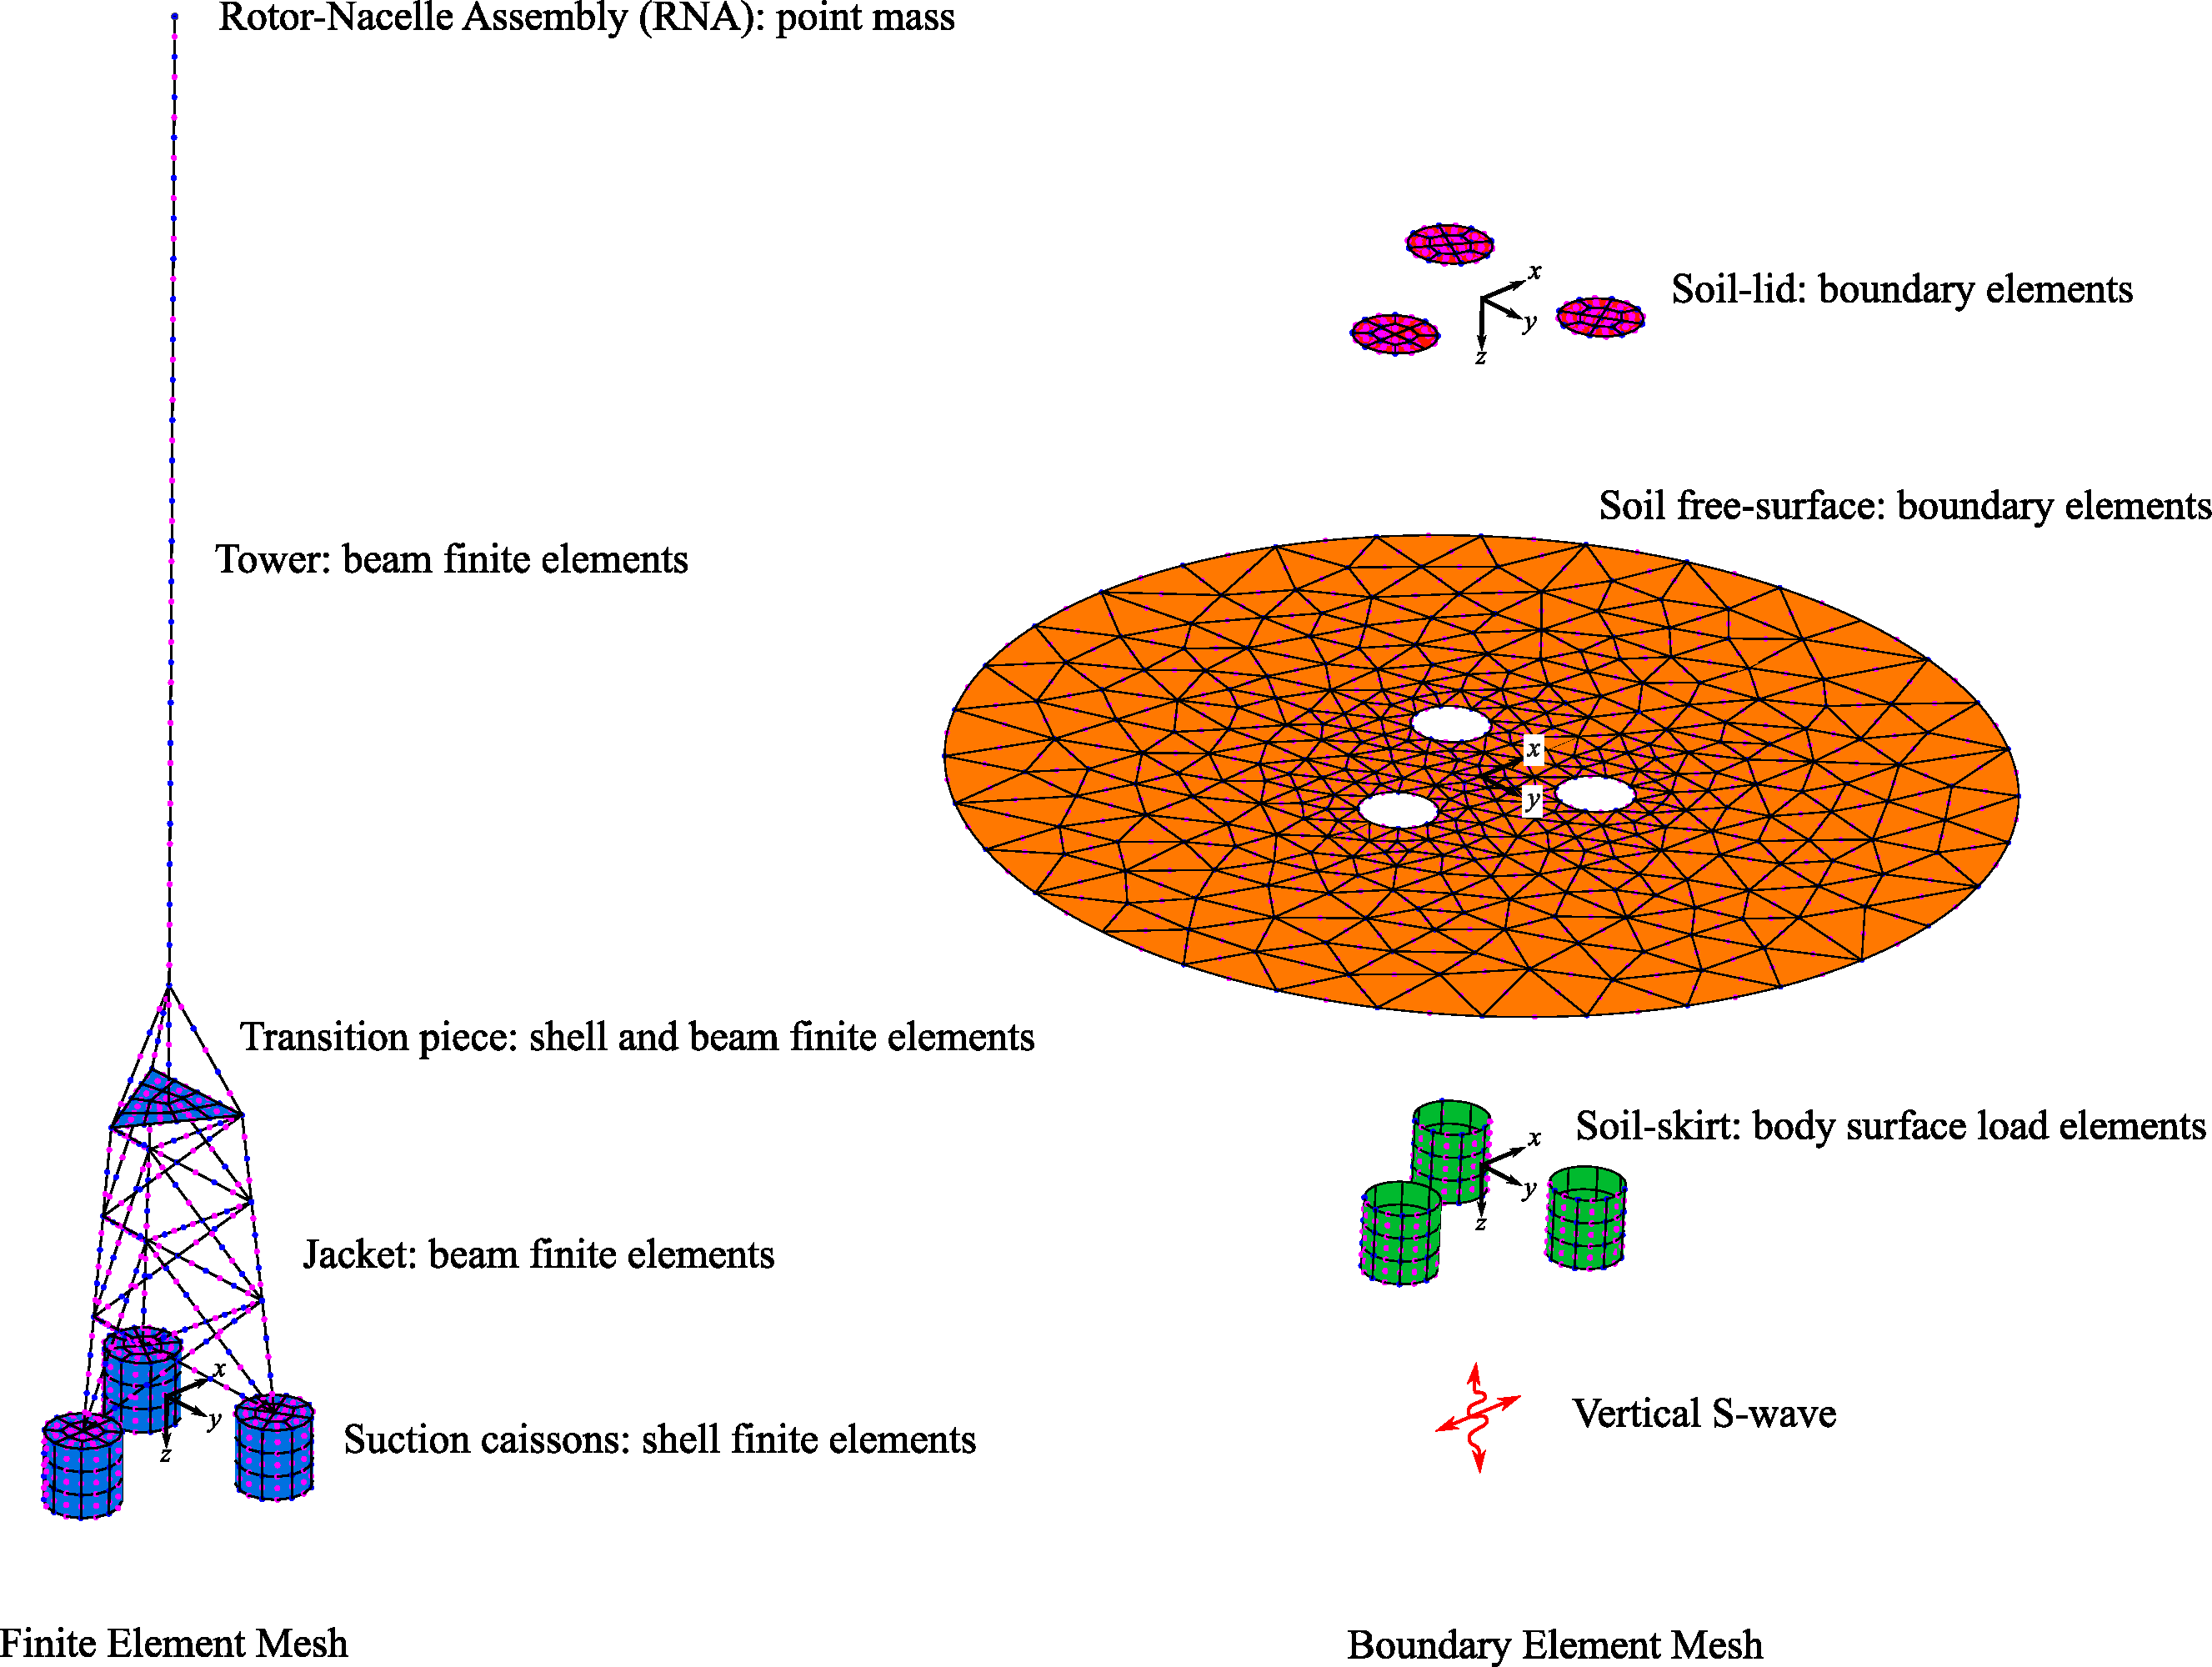
\includegraphics[scale=0.35]{owt_model_flexible.pdf}
	\caption{Geometry for the FEM-BEM model.}
	\label{fig:geometry2}
\end{figure}

\section{Pre-processing}

\subsection{Mesh generation with Gmsh}

\subsubsection{GEO file}
In this model several parts of the offshore wind turbine were also defined in the *.geo file: Jacket joints, Jacket members, Transition piece, Tower, Foundation (suction caissons) and Free Surface. For the Foundation and the Free Surface, auxiliary files were created and imported into the main file "mesh.geo". These auxiliary files allowed to define the target parts by using different functions, loops and macros. For example, the customized functions were built by setting the command "Function" followed by a name and then by ending with the command "Return", the function "Geometry.AutoCoherence = 0" helps to prevent any automatic duplicate check or replacement, the variable name "newp", "newl", "newll" and "news" select new line, line loop, surface and surface tags, the function "Atan2" calculates the arc tangent of the first value divided by the second one, the function "Rotate" turns elements by giving an angle of radians, the direction of rotation and a point on the axis of rotation, 

The remaining functions have been already explained in previous tutorials.

\begin{figure}[tbh!]
	\centering
	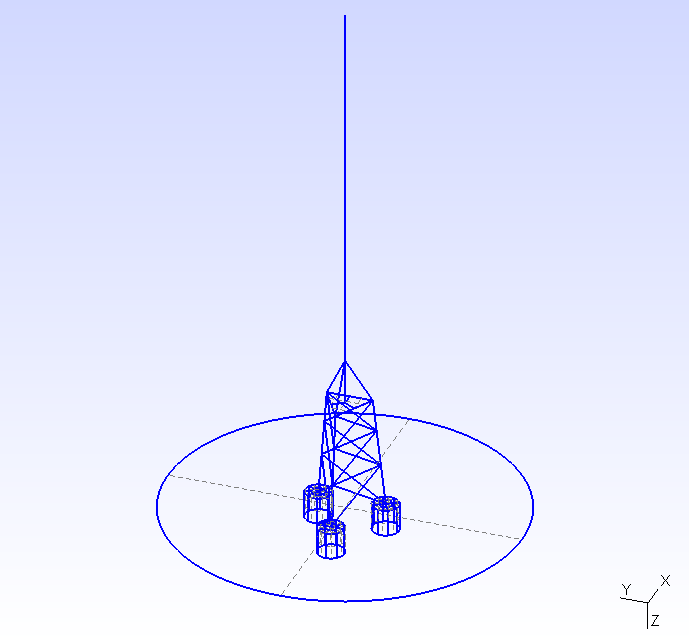
\includegraphics[scale=0.6]{geo2.png}
	\caption{Geometry for the BEM-FEM model resulting from the *.geo file.}
	\label{fig:geo2}
\end{figure}

\subsubsection{MSH file}

The mesh is shown in Figure \ref{fig:mesh2}.

\begin{figure}[h!]
	\centering
	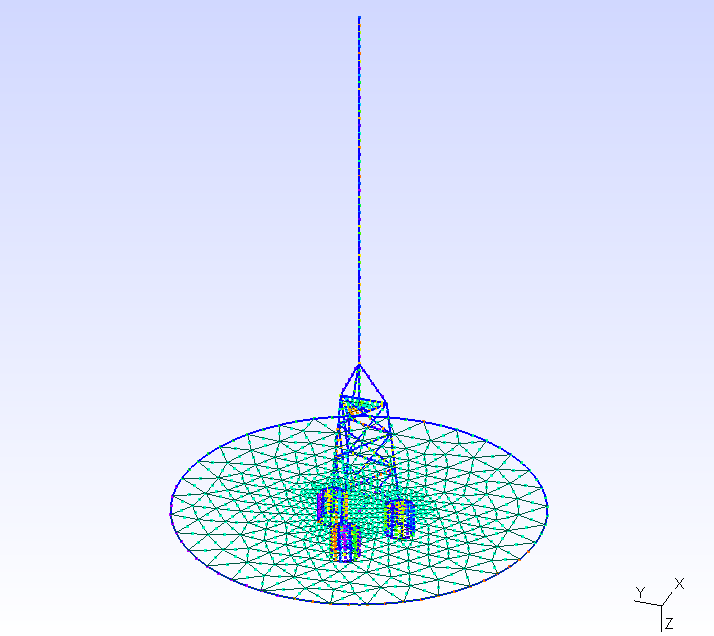
\includegraphics[scale=0.6]{mesh2.png}
	\caption{Mesh for the BEM-FEM model resulting from the *.geo file.}
	\label{fig:mesh2}
\end{figure}

\subsection{Input data file}

The principal difference of the BEM-FEM model with respect to the FEM model is the existence of incident waves.

In the section [incident waves], the incoming waves are defined. Note that in this example the geometry is defined with the z-axis oriented downwards. It is of course not mandatory to define the global axes this way. In fact, the geometry can be built defining the z-axis as oriented either downwards or upwards. However, this detail affects the way in which the incident field can be defined because, at the moment, the two routines implemented for the definition of the incident field (corresponding to a homogenous or a multilayered half-space) have different assumptions and restrictions:

\begin{itemize}
	\item The routine that implements the homogeneous half-space incident field only works when the positive z-axis goes outside the half-space\footnote{See Tutorials 7b and 11.}.
	
	\item The routine that implements the multilayered half-space incident field is more general and allows both upwards and downwords z-axis orientations.
\end{itemize}

Taking into consideration the abovementioned comments, the format of this section for the present example is the following multilayered routine:

The format has a first line for the number of waves (1), a second line for the wave identifier (1), a third line for the wave class (plane), a fourth line for the space ("multilayered\_half-space" with $np = -3$; number of layers = 2; z top coordinates of the layers = 0, 100; materials of the layers = 1, 2; the same number of 1s and (0.,0.)s as layers), a fifth line for the variable (0 for displacement), the amplitude (1.,0.), the reference point ($ x0(1) = 0 $, $ x0(2) = 0 $, $ x0(3) = 0 $)  and the angles ($ varphi = 0 $, $ theta = 90 $), a sixth line for symmetry options ($ xs(1) = 0 $, $ xs(2) = 0 $, $ xs(3) = 0 $, $ symconf(1) = 0 $, $ symconf(2) = 0 $, $ symconf(3) = 0 $) and a seventh line for the region type (viscoelastic) and the wave type (sh). This data input is intended to further generalize the incident field, but the corresponding functions are not yet implemented and that is why the input has this format. 

\begin{Verbatim}
[incident waves]
1
1
plane
multilayered_half-space -3 2 0 100 1 2 1 1 (0.,0.) (0.,0.)
0 (1.,0.) 0. 0. 0. 0. 90.
0. 0. 0. 0. 0. 0.
viscoelastic sh
\end{Verbatim}

The whole data file applied to the problem is the following:

\begin{Verbatim}
[problem]
type = mechanics
analysis = harmonic
n = 3D

[frequencies]
Hz
lin
200
0.01
10

[settings]
mesh_file_mode = 2 "mesh.msh"

[export]
complex_notation = cartesian
real_format=eng_simple

[materials]
4
1 elastic_solid rho 7850 E 2.1e+11 nu 0.3 xi 0.005
2 elastic_solid rho 1800 mu 5.832e+07 nu 0.35 xi 0.05
3 elastic_solid rho 1800 mu 5.832e+07 nu 0.35 xi 0.05
4 elastic_solid rho 7850 E 2.1e+14 nu 0.3 xi 0.005

[fe subregions]
34
2 2 0 0
3 3 0 0
4 4 0 0
5 5 0 0
6 6 0 0
7 7 0 0
8 8 0 0
9 9 0 0
10 10 0 0
11 11 0 0
12 12 0 0
13 13 0 0
14 14 0 0
15 15 0 0
16 16 0 0
17 17 0 0
18 18 0 0
19 19 0 0
20 20 0 0
21 21 0 0
22 22 0 0
23 23 0 0
24 24 0 0
25 25 0 0
26 26 0 0
27 27 0 0
28 28 0 0
29 29 0 0
30 30 0 0
31 31 0 0
32 32 0 0
33 33 0 0
34 34 0 0
35 35 0 0

[be body loads]
1
1 37

[boundaries]
2
1 36 ordinary
2 38 ordinary

[regions]
3

1 fe
33 2 3 4 5 6 7 8 9 10 11 12 13 14 15 16 17 18 19 20 21 22 23 24 25 26 27 28 29 30 31 32 33 35 
material 1

2 be
2 1 2
material 2
1 1
1 1

3 fe
1 34
material 4

[cross sections]
36
strbeam_t 1 2 hollow_circle 1.94446 1.87919 0. 1. 0.
strbeam_t 1 3 hollow_circle 0.733395 0.708775 0. 1. 0.
strbeam_t 1 4 hollow_circle 0.773882 0.747903 0. 1. 0.
strbeam_t 1 5 hollow_circle 0.846749 0.818324 0. 1. 0.
strbeam_flooded 4 2 3 4 5 -20 0 1027
strbeam_submerged 4 2 3 4 5 -20 0 1027
degshell 1 6 0.2
strbeam_t 1 7 hollow_circle 1.94446 1.87919 0. 1. 0.
strbeam_t 1 8 hollow_circle 8.14706 8.07303 0. 1. 0.
strbeam_t 1 9 hollow_circle 7.94216 7.87076 0. 1. 0.
strbeam_t 1 10 hollow_circle 7.83824 7.76817 0. 1. 0.
strbeam_t 1 11 hollow_circle 7.73431 7.66559 0. 1. 0.
strbeam_t 1 12 hollow_circle 7.63039 7.563 0. 1. 0.
strbeam_t 1 13 hollow_circle 7.52647 7.46042 0. 1. 0.
strbeam_t 1 14 hollow_circle 7.42255 7.35783 0. 1. 0.
strbeam_t 1 15 hollow_circle 7.31863 7.25525 0. 1. 0.
strbeam_t 1 16 hollow_circle 7.21471 7.15266 0. 1. 0.
strbeam_t 1 17 hollow_circle 7.11078 7.05007 0. 1. 0.
strbeam_t 1 18 hollow_circle 7.00686 6.94749 0. 1. 0.
strbeam_t 1 19 hollow_circle 6.90294 6.8449 0. 1. 0.
strbeam_t 1 20 hollow_circle 6.79902 6.74232 0. 1. 0.
strbeam_t 1 21 hollow_circle 6.6951 6.63973 0. 1. 0.
strbeam_t 1 22 hollow_circle 6.59118 6.53715 0. 1. 0.
strbeam_t 1 23 hollow_circle 6.48725 6.43456 0. 1. 0.
strbeam_t 1 24 hollow_circle 6.38333 6.33198 0. 1. 0.
strbeam_t 1 25 hollow_circle 6.27941 6.22939 0. 1. 0.
strbeam_t 1 26 hollow_circle 6.17549 6.12681 0. 1. 0.
strbeam_t 1 27 hollow_circle 6.07157 6.02422 0. 1. 0.
strbeam_t 1 28 hollow_circle 5.96765 5.92163 0. 1. 0.
strbeam_t 1 29 hollow_circle 5.86373 5.81905 0. 1. 0.
strbeam_t 1 30 hollow_circle 5.7598 5.71646 0. 1. 0.
strbeam_t 1 31 hollow_circle 5.65588 5.61388 0. 1. 0.
strbeam_t 1 32 hollow_circle 5.55196 5.51129 0. 1. 0.
degshell 1 34 0.164
degshell 1 35 0.082
pmass 1 33 unbalanced 770180 0 0 0 0 0 0 770180 0 0 0 0 0 0 770180 0 0 0 0 0 0 0 0 0 
0 0 0 0 0 0 0 0 0 0 0 0 

[incident waves]
1
1
plane
multilayered_half-space -3 2 0 100 1 2 1 1 (0.,0.) (0.,0.)
0 (1.,0.) 0. 0. 0. 0. 90.
0. 0. 0. 0. 0. 0.
viscoelastic sh
\end{Verbatim}

\part{Results and discussion}

\section{Comments}

Figure \ref{fig:results} shows the Rotor-Nacelle Assembly (RNA) displacement for the FEM model (rigid base) and the BEM-FEM model (flexible base).

\begin{figure}[tbh!]
	\centering
	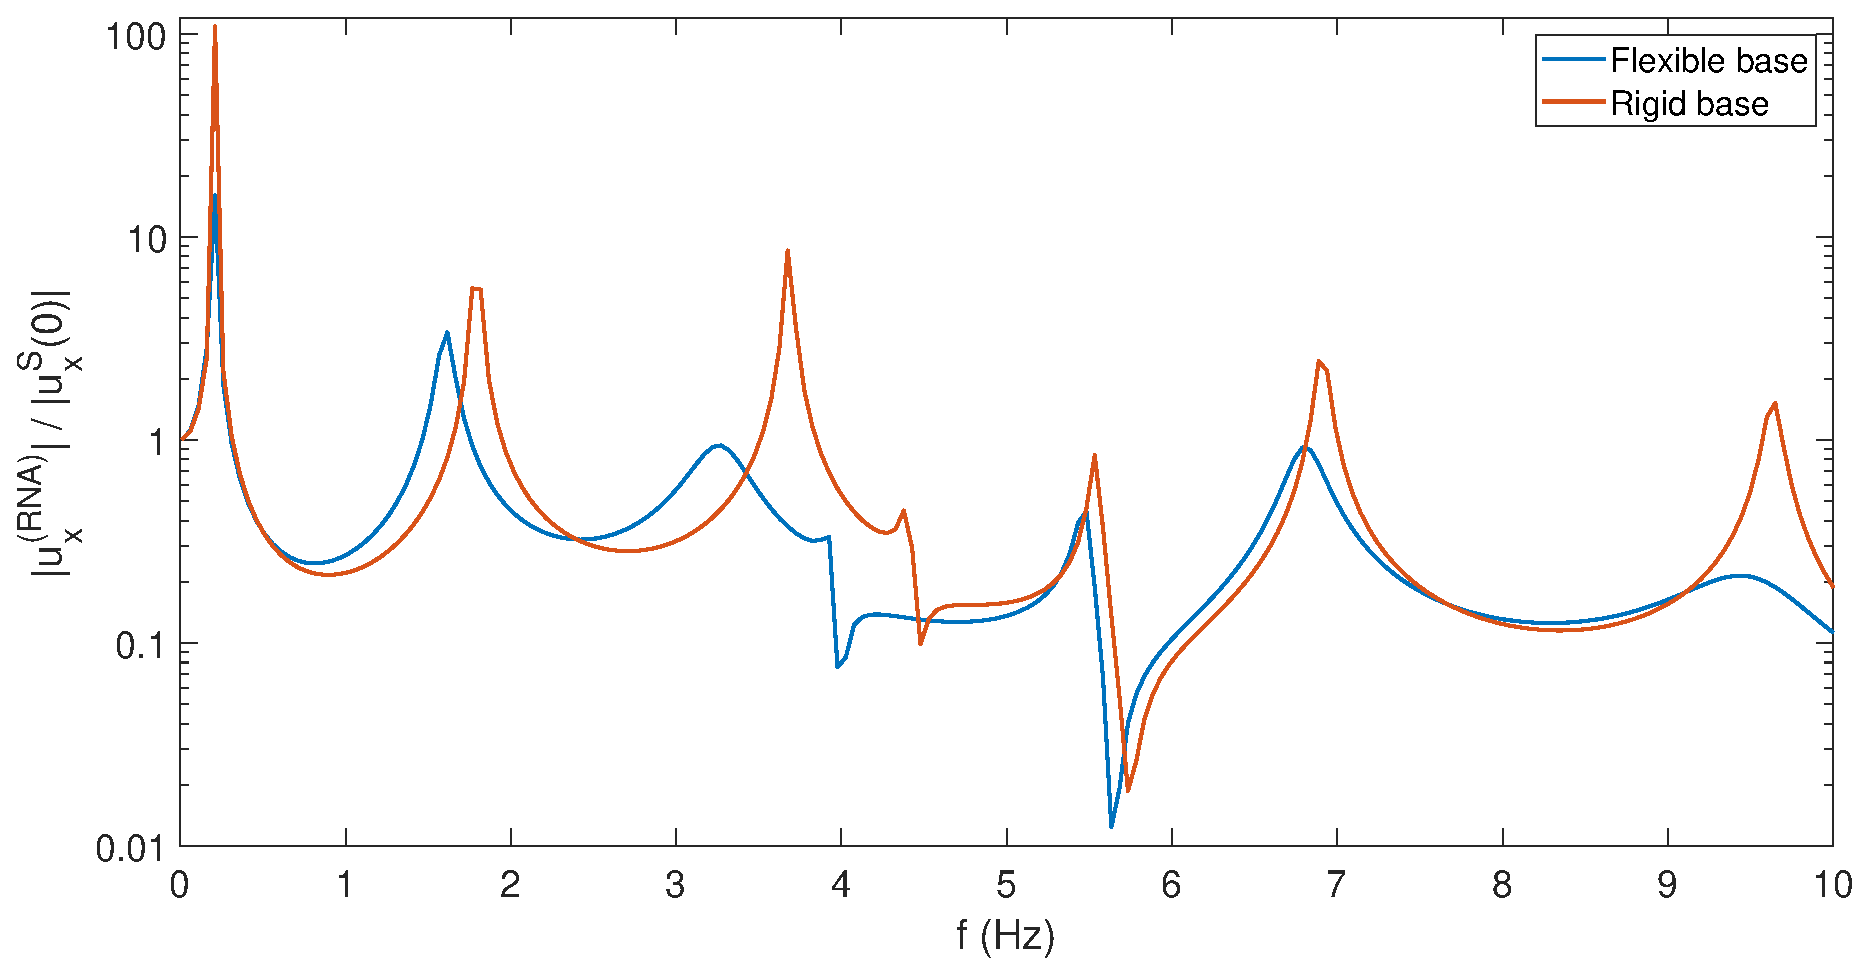
\includegraphics[scale=0.5]{wind_turbine.eps}
	\caption{Rotor-Nacelle Assembly (RNA) displacement for the FEM model (rigid base) and the BEM-FEM model (flexible base).}
	\label{fig:results}
\end{figure}

\FloatBarrier

\begin{thebibliography}{99}
	
	\bibitem{gmsh} C. Geuzaine and J.-F. Remacle, "Gmsh: a three-dimensional finite element mesh generator with built-in pre- and post-processing facilities." \emph{International Journal for Numerical Methods in Engineering}, Volume 79, Issue 11, pages 1309--1331, (2009)
	
	\bibitem{gmshweb} C. Geuzaine and J.-F. Remacle, "Gmsh." \url{http://gmsh.info/}

\end{thebibliography}

\end{document}
